\documentclass[
  11pt,
  letterpaper,
   addpoints,
   answers
  ]{exam}

\usepackage{../exercise-preamble}
\usepackage{float}
\usepackage{tikz}
\usetikzlibrary{decorations.pathmorphing}

\begin{document}
\pagestyle{headandfoot}
\firstpagefooter{ }{Página \thepage\ de \numpages}{ }
\runningfooter{ }{Página \thepage\ de \numpages}{ }

\noindent
\begin{minipage}{0.47\textwidth}

\includegraphics[width=\textwidth]{../fcfm_die.png}
\end{minipage}
\begin{minipage}{0.53\textwidth}
\begin{center} 
\large\textbf{Introducción a la Física Moderna} (F1100-5) \\
\large\textbf{Clase auxiliar 5} \\
\normalsize Prof.~ Rodrigo Soto.\\
\normalsize Prof.~Aux.~Erik Sáez - Javiera Toro 
\end{center}
\end{minipage}

\vspace{0.5cm}
\noindent
\vspace{.85cm}

\begin{questions}
%--------------------------
\noindent
\begin{minipage}[t]{0.6\textwidth}
\question Un péndulo de longitud $L$ con una masa $M$ está unido lateralmente a un resorte de constante elástica $k$, como se muestra esquemáticamente. Cuando la masa cuelga verticalmente bajo el punto de suspensión, el resorte está sin deformación.
\begin{parts}
  \part Obtén una expresión aproximada para el período de oscilación del sistema para pequeñas amplitudes (linealiza las ecuaciones de movimiento).
  \part Supón $M=1{,}00\,\mathrm{kg}$ y que, en ausencia del resorte, el período del péndulo es $2{,}00\,\mathrm{s}$. Determina $k$ si el período del sistema acoplado es $1{,}00\,\mathrm{s}$.
\end{parts}
\end{minipage}%
\hfill
\begin{minipage}[t]{0.38\textwidth}
\centering
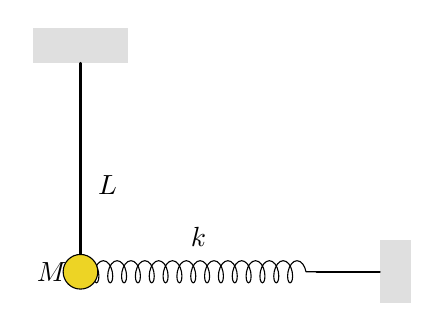
\begin{tikzpicture}[x=1cm,y=1cm,line cap=round,line join=round,>=latex,baseline=(current bounding box.north)]
  % Parameters
  \def\L{2.2}
  \def\spr{3.0}

  % Supports (simple blocks)
  \fill[gray!25] (-0.6,\L+0.45) rectangle (0.6,\L+0.9);
  \fill[gray!25] (\spr+0.8,-0.4) rectangle (\spr+1.2,0.4);

  % Hook and string
  \draw[thick] (0,\L+0.45) -- (0,\L);
  \draw[thick] (0,\L) -- (0,0);

  % Spring to the right
  \draw[decorate,decoration={coil,segment length=5pt,amplitude=4pt}]
    (0,0) -- (\spr,0);
  % Small rod to wall
  \draw[thick] (\spr,0) -- (\spr+0.8,0);

  % Bob (draw last to be in front of the spring)
  \fill[yellow!70!brown, draw=black] (0,0) circle (0.22);
  \node[left] at (-0.05,0) {$M$};

  % Labels
  \node[right] at (0.1,\L/2) {$L$};
  \node[above] at (\spr/2,0.2) {$k$};
\end{tikzpicture}
\end{minipage}
%-------------------------
\begin{solution}
  \subsection*{Resolución 1.1}
  
  Para resolver este problema, necesitamos establecer las ecuaciones de movimiento del sistema péndulo-resorte.
  
  Sea $\theta$ el ángulo que forma la cuerda con la vertical. Las coordenadas de la masa son:
  \begin{align}
    x &= L\sin\theta \\
    y &= -L\cos\theta
  \end{align}
  
  La energía cinética del sistema es:
  \begin{equation}
    T = \frac{1}{2}M(\dot{x}^2 + \dot{y}^2) = \frac{1}{2}ML^2\dot{\theta}^2
  \end{equation}
  
  La energía potencial tiene dos contribuciones: gravitacional y elástica:
  \begin{align}
    V &= MgL(1-\cos\theta) + \frac{1}{2}kx^2 \\
    &= MgL(1-\cos\theta) + \frac{1}{2}kL^2\sin^2\theta
  \end{align}
  
  Para pequeñas oscilaciones, usamos las aproximaciones $\sin\theta \approx \theta$ y $\cos\theta \approx 1 - \frac{\theta^2}{2}$:
  \begin{equation}
    V \approx \frac{1}{2}MgL\theta^2 + \frac{1}{2}kL^2\theta^2 = \frac{1}{2}(MgL + kL^2)\theta^2
  \end{equation}
  
  El Lagrangiano es:
  \begin{equation}
    \mathcal{L} = T - V = \frac{1}{2}ML^2\dot{\theta}^2 - \frac{1}{2}(MgL + kL^2)\theta^2
  \end{equation}
  
  La ecuación de Euler-Lagrange nos da:
  \begin{equation}
    ML^2\ddot{\theta} + (MgL + kL^2)\theta = 0
  \end{equation}
  
  Simplificando:
  \begin{equation}
    \ddot{\theta} + \frac{g}{L}\left(1 + \frac{kL}{Mg}\right)\theta = 0
  \end{equation}
  
  Esta es la ecuación de un oscilador armónico simple con frecuencia angular:
  \begin{equation}
    \omega = \sqrt{\frac{g}{L}\left(1 + \frac{kL}{Mg}\right)}
  \end{equation}
  
  Por tanto, el período de oscilación es:
  \begin{equation}
    \boxed{T = 2\pi\sqrt{\frac{L}{g\left(1 + \frac{kL}{Mg}\right)}}}
  \end{equation}
  
  \subsection*{Resolución 1.2}
  
  Datos del problema:
  \begin{itemize}
    \item $M = 1{,}00\,\mathrm{kg}$
    \item Período sin resorte: $T_0 = 2{,}00\,\mathrm{s}$
    \item Período con resorte: $T = 1{,}00\,\mathrm{s}$
  \end{itemize}
  
  Del período del péndulo simple sin resorte:
  \begin{equation}
    T_0 = 2\pi\sqrt{\frac{L}{g}} = 2{,}00\,\mathrm{s}
  \end{equation}
  
  De aquí obtenemos:
  \begin{equation}
    \frac{L}{g} = \left(\frac{T_0}{2\pi}\right)^2 = \left(\frac{2{,}00}{2\pi}\right)^2 = \frac{1}{\pi^2}\,\mathrm{s^2}
  \end{equation}
  
  Con el resorte, el período es:
  \begin{equation}
    T = 2\pi\sqrt{\frac{L}{g\left(1 + \frac{kL}{Mg}\right)}} = 1{,}00\,\mathrm{s}
  \end{equation}
  
  Dividiendo las ecuaciones:
  \begin{equation}
    \frac{T}{T_0} = \frac{1}{\sqrt{1 + \frac{kL}{Mg}}} = \frac{1{,}00}{2{,}00} = \frac{1}{2}
  \end{equation}
  
  Elevando al cuadrado:
  \begin{equation}
    \frac{1}{4} = \frac{1}{1 + \frac{kL}{Mg}}
  \end{equation}
  
  Despejando:
  \begin{equation}
    1 + \frac{kL}{Mg} = 4 \quad \Rightarrow \quad \frac{kL}{Mg} = 3
  \end{equation}
  
  Por tanto:
  \begin{equation}
    k = \frac{3Mg}{L}
  \end{equation}
  
  Necesitamos encontrar $L$. De $\frac{L}{g} = \frac{1}{\pi^2}$:
  \begin{equation}
    L = \frac{g}{\pi^2} = \frac{9{,}81}{\pi^2} \approx 0{,}994\,\mathrm{m}
  \end{equation}
  
  Finalmente:
  \begin{equation}
    k = \frac{3 \times 1{,}00 \times 9{,}81}{0{,}994} \approx 29{,}6\,\mathrm{N/m}
  \end{equation}
  
  \begin{equation}
    \boxed{k \approx 29{,}6\,\mathrm{N/m}}
  \end{equation}
\end{solution}
%--------------------------
\question 
\begin{parts}
  \part Bosquee la función
  \begin{equation}
    f(x) = \frac{1\,\mathrm{cm}}{1 + \left(x/1\,\mathrm{cm}\right)^2}.
  \end{equation}
  Escriba $f(\bar{x})$ para $\bar{x} = x - ct$, donde $c$ es la velocidad de propagación de la onda y $t$ el tiempo. Si $c = 1\,\mathrm{cm/s}$, bosquee la función $u(x,t) = f(x-ct)$ para $t = 0, 1, 2\,\mathrm{s}$, donde $u(x,t)$ representa la amplitud de la onda en la posición $x$ y tiempo $t$.

  \part Calcule la velocidad vertical $v(x,t)$ de la cuerda en el instante $t = 0$. Para esto, derive la función $u(x,t)$ con respecto al tiempo considerando $x$ constante.

  \part Grafique $v(x,0)$ en función de $x$. Note que esta es positiva y negativa en ciertas partes. Interprete el resultado.
\end{parts}

\begin{solution}
  \subsection*{Resolución 2.1}
  
  La función dada es:
  \begin{equation}
    f(x) = \frac{1\,\mathrm{cm}}{1 + \left(x/1\,\mathrm{cm}\right)^2}
  \end{equation}
  
  Esta es una función de tipo Lorentziana centrada en $x = 0$ con amplitud máxima de $1\,\mathrm{cm}$ y ancho característico de $1\,\mathrm{cm}$.
  
  Para $\bar{x} = x - ct$, la función se convierte en:
  \begin{equation}
    f(\bar{x}) = f(x-ct) = \frac{1\,\mathrm{cm}}{1 + \left((x-ct)/1\,\mathrm{cm}\right)^2}
  \end{equation}
  
  Por tanto:
  \begin{equation}
    u(x,t) = f(x-ct) = \frac{1\,\mathrm{cm}}{1 + \left((x-ct)/1\,\mathrm{cm}\right)^2}
  \end{equation}
  
  Con $c = 1\,\mathrm{cm/s}$:
  \begin{align}
    u(x,t) &= \frac{1\,\mathrm{cm}}{1 + (x-t)^2/\mathrm{cm}^2} \\
    &= \frac{1\,\mathrm{cm}}{1 + (x-t)^2\,\mathrm{cm}^{-2}}
  \end{align}
  
  Para los tiempos específicos:
  \begin{align}
    t = 0\,\mathrm{s}: \quad u(x,0) &= \frac{1\,\mathrm{cm}}{1 + x^2\,\mathrm{cm}^{-2}} \\
    t = 1\,\mathrm{s}: \quad u(x,1) &= \frac{1\,\mathrm{cm}}{1 + (x-1\,\mathrm{cm})^2\,\mathrm{cm}^{-2}} \\
    t = 2\,\mathrm{s}: \quad u(x,2) &= \frac{1\,\mathrm{cm}}{1 + (x-2\,\mathrm{cm})^2\,\mathrm{cm}^{-2}}
  \end{align}
  
  El pulso se propaga hacia la derecha con velocidad $c = 1\,\mathrm{cm/s}$, manteniendo su forma.
  
  \subsection*{Resolución 2.2}
  
  Para calcular la velocidad vertical, derivamos $u(x,t)$ con respecto al tiempo:
  \begin{equation}
    v(x,t) = \frac{\partial u(x,t)}{\partial t}
  \end{equation}
  
  Usando la regla de la cadena:
  \begin{equation}
    u(x,t) = \frac{1\,\mathrm{cm}}{1 + (x-ct)^2\,\mathrm{cm}^{-2}}
  \end{equation}
  
  Sea $\xi = x - ct$, entonces:
  \begin{equation}
    \frac{\partial u}{\partial t} = \frac{du}{d\xi} \cdot \frac{\partial \xi}{\partial t} = \frac{du}{d\xi} \cdot (-c)
  \end{equation}
  
  Calculando la derivada:
  \begin{align}
    \frac{du}{d\xi} &= \frac{d}{d\xi}\left[\frac{1\,\mathrm{cm}}{1 + \xi^2\,\mathrm{cm}^{-2}}\right] \\
    &= 1\,\mathrm{cm} \cdot \frac{d}{d\xi}\left[(1 + \xi^2\,\mathrm{cm}^{-2})^{-1}\right] \\
    &= 1\,\mathrm{cm} \cdot (-1)(1 + \xi^2\,\mathrm{cm}^{-2})^{-2} \cdot 2\xi\,\mathrm{cm}^{-2} \\
    &= -\frac{2\xi\,\mathrm{cm}^{-1}}{(1 + \xi^2\,\mathrm{cm}^{-2})^2}
  \end{align}
  
  Por tanto:
  \begin{equation}
    v(x,t) = -(-c) \cdot \frac{2(x-ct)\,\mathrm{cm}^{-1}}{[1 + (x-ct)^2\,\mathrm{cm}^{-2}]^2} = \frac{2c(x-ct)\,\mathrm{cm}^{-1}}{[1 + (x-ct)^2\,\mathrm{cm}^{-2}]^2}
  \end{equation}
  
  En $t = 0$ y con $c = 1\,\mathrm{cm/s}$:
  \begin{equation}
    v(x,0) = \frac{2x\,\mathrm{cm}^{-1}}{[1 + x^2\,\mathrm{cm}^{-2}]^2}
  \end{equation}
  
  \subsection*{Resolución 2.3}
  
  La función $v(x,0)$ tiene las siguientes características:
  
  \begin{itemize}
    \item Para $x > 0$: $v(x,0) > 0$ (velocidad hacia arriba)
    \item Para $x < 0$: $v(x,0) < 0$ (velocidad hacia abajo)  
    \item Para $x = 0$: $v(0,0) = 0$ (velocidad nula)
  \end{itemize}
  
  La velocidad máxima positiva ocurre en:
  \begin{equation}
    \frac{dv}{dx}\bigg|_{x=x_{\max}} = 0
  \end{equation}
  
  Resolviendo se obtiene $x_{\max} = 1/\sqrt{3}\,\mathrm{cm} \approx 0{,}577\,\mathrm{cm}$ con velocidad máxima:
  \begin{equation}
    v_{\max} = v\left(\frac{1}{\sqrt{3}}\,\mathrm{cm}, 0\right) = \frac{\sqrt{3}}{4}\,\mathrm{s}^{-1} \approx 0{,}433\,\mathrm{s}^{-1}
  \end{equation}
  
  **Interpretación física**: La velocidad vertical describe cómo se mueve cada punto de la cuerda en el instante $t = 0$. El patrón antisimétrico ($v(-x,0) = -v(x,0)$) indica que el pulso se está propagando hacia la derecha. Los puntos a la derecha del centro se mueven hacia arriba (preparando el terreno para el pulso que llega), mientras que los puntos a la izquierda se mueven hacia abajo (regresando a la posición de equilibrio después de que el pulso ha pasado).
\end{solution}

%--------------------------
\question Se tiene una masa $m$ sostenida de dos cuerdas de largos $L_1$ y $L_2$, con tensiones $T_1$ y $T_2$ respectivamente en presencia de gravedad, como se observa en la figura. Considere que $T_2$ es conocido y $T_1$ es tal que el sistema no se mueve verticalmente.

Si inicialmente la masa se suelta desde el reposo a una distancia $x$,
\begin{parts}
  \part Calcule el valor de $T_1$ para que el sistema no se mueva verticalmente.
  \part Encuentre la frecuencia angular de oscilación.
  \part Calcule el período de oscilación.
  \part Calcule la amplitud de oscilación de la masa.
\end{parts}
Considere para sus cálculos y aproximaciones $x \ll L_1, L_2$, y que las tensiones se mantienen al deformarse la cuerda.
\begin{figure}[H]
\centering
\begin{tikzpicture}[%
    >=Latex,
    board/.style={line width=2.6pt, draw=brown!70!black, line cap=round},
    stringV/.style={line width=1.4pt, draw=blue!70!black},
    string/.style={line width=1.4pt, draw=gray!70!black},
    mass/.style={draw=red!70!black, fill=red!70, line width=0.5pt},
    note/.style={scale=0.9}
]

% ------------------- Panel izquierdo: cuerda vertical -------------------
\def\H{3}    % altura entre barras
\def\W{3}    % ancho de barras
\def\xs{1}   % x de la cuerda
\def\ym{1.5} % y de la masa
\def\r{0.14} % radio de la masa

% Barras
\draw[board] (0,\H) -- (\W,\H);
\draw[board] (0,0)  -- (\W,0);

% Cuerda vertical
\draw[stringV] (\xs,0) -- (\xs,\H);

% Masa (por encima de la cuerda)
\fill[mass] (\xs,\ym) circle (\r);
\node[anchor=west] at (\xs+\r+0.08,\ym) {$m$};

% Tensiones T1 y T2
\node[note,blue!70!black,anchor=west] at (\xs+0.18, {(\H+\ym)/2}) {T1};
\node[note,blue!70!black,anchor=west] at (\xs+0.18, {\ym/2})      {T2};

% Brazos L1 y L2 con llaves
\draw[decorate,decoration={brace,mirror,amplitude=4pt}]
  ([xshift=-0.32cm]\xs,\ym) -- ([xshift=-0.32cm]\xs,\H)
  node[midway,left=6pt,note] {L1};
\draw[decorate,decoration={brace,mirror,amplitude=4pt}]
  ([xshift=-0.32cm]\xs,0) -- ([xshift=-0.32cm]\xs,\ym)
  node[midway,left=6pt,note] {L2};

% ------------------- Panel derecho: masa desplazada -------------------
\begin{scope}[xshift=6.2cm]
  % Barras
  \draw[board] (0,\H) -- (\W,\H);
  \draw[board] (0,0)  -- (\W,0);

  % Línea de referencia vertical
  \draw[stringV,dashed] (\xs,0) -- (\xs,\H);

  % Coordenadas clave
  \coordinate (Top) at (\xs,\H);
  \coordinate (Bot) at (\xs,0);
  \coordinate (M)   at (\xs+0.70,\ym); % masa desplazada

  % Cuerdas inclinadas (detrás de la masa)
  \draw[string] (Top) -- (M);
  \draw[string] (Bot) -- (M);

  % Etiquetas T1 y T2
  \node[note,anchor=west] at ($(Top)!0.58!(M)+(0.10,0.00)$) {T1};
  \node[note,anchor=west] at ($(Bot)!0.58!(M)+(0.10,0.00)$) {T2};

  % Flecha x (debajo de la masa y acortada al borde)
  \draw[->,thick,green!60!black,shorten >=\r+0.02]
    (\xs,\ym) -- (M) node[midway,above,note] {$x$};

  % Doble referencia L1/L2 (solo texto)
  \node[note] at (-0.35, {(\H+\ym)/2}) {L1};
  \node[note] at (-0.35, {\ym/2})      {L2};

  % Masa dibujada al final (encima de cuerdas y flecha)
  \fill[mass] (M) circle (\r);
  \node[anchor=west] at ($(M)+(\r+0.08,0)$) {$m$};
\end{scope}

% ------------------- Flecha de gravedad -------------------
\draw[->,line width=1.1pt] (11.0,2.6) -- (11.0,0.6) node[anchor=west] {$\vec g$};

\end{tikzpicture}
\caption{Masa sostenida por dos cuerdas con tensiones $T_1$ y $T_2$.}
\end{figure}
%--------------------------
\end{questions}
\end{document}